% !TEX TS-program = pdflatex
% !TEX encoding = UTF-8 Unicode

% This is a simple template for a LaTeX document using the "article" class.
% See "book", "report", "letter" for other types of document.

\documentclass[11pt]{article} % use larger type; default would be 10pt

\usepackage[utf8]{inputenc} % set input encoding (not needed with XeLaTeX)

%%% Examples of Article customizations
% These packages are optional, depending whether you want the features they provide.
% See the LaTeX Companion or other references for full information.

%%% PAGE DIMENSIONS
\usepackage{geometry} % to change the page dimensions
\geometry{a4paper} % or letterpaper (US) or a5paper or....
% \geometry{margin=2in} % for example, change the margins to 2 inches all round
% \geometry{landscape} % set up the page for landscape
%   read geometry.pdf for detailed page layout information

\usepackage{graphicx} % support the \includegraphics command and options

% \usepackage[parfill]{parskip} % Activate to begin paragraphs with an empty line rather than an indent

%%% PACKAGES
\usepackage{booktabs} % for much better looking tables
\usepackage{array} % for better arrays (eg matrices) in maths
\usepackage{paralist} % very flexible & customisable lists (eg. enumerate/itemize, etc.)
\usepackage{verbatim} % adds environment for commenting out blocks of text & for better verbatim
\usepackage{subfig} % make it possible to include more than one captioned figure/table in a single float
% These packages are all incorporated in the memoir class to one degree or another...

%%% HEADERS & FOOTERS
\usepackage{fancyhdr} % This should be set AFTER setting up the page geometry
\pagestyle{fancy} % options: empty , plain , fancy
\renewcommand{\headrulewidth}{0pt} % customise the layout...
\lhead{}\chead{}\rhead{}
\lfoot{}\cfoot{\thepage}\rfoot{}

\usepackage{multirow}
\usepackage{algorithm}
\usepackage{algorithmic}
%\usepackage{multicol}

%%% SECTION TITLE APPEARANCE
\usepackage{sectsty}
\allsectionsfont{\sffamily\mdseries\upshape} % (See the fntguide.pdf for font help)
% (This matches ConTeXt defaults)

%%% ToC (table of contents) APPEARANCE
\usepackage[nottoc,notlof,notlot]{tocbibind} % Put the bibliography in the ToC
\usepackage[titles,subfigure]{tocloft} % Alter the style of the Table of Contents
\renewcommand{\cftsecfont}{\rmfamily\mdseries\upshape}
\renewcommand{\cftsecpagefont}{\rmfamily\mdseries\upshape} % No bold!

%%% END Article customizations

%%% The "real" document content comes below...

\title{Supplementary material}
%\author{The Author}
\date{} % Activate to display a given date or no date (if empty),
         % otherwise the current date is printed 

\begin{document}
\maketitle

\section{Task hierarchies}

 \begin{figure*}[ht]
 \begin{tabular}{cc}
 %\hspace{-1in}\includegraphics[scale=0.6]{Taxi-Hierarchy.pdf} &
 %\hspace{-2.5in}\includegraphics[scale=0.6]{Wargus-Hierarchy.pdf}\\
 %\vspace{-5.2in}
 & \multirow{2}{*}{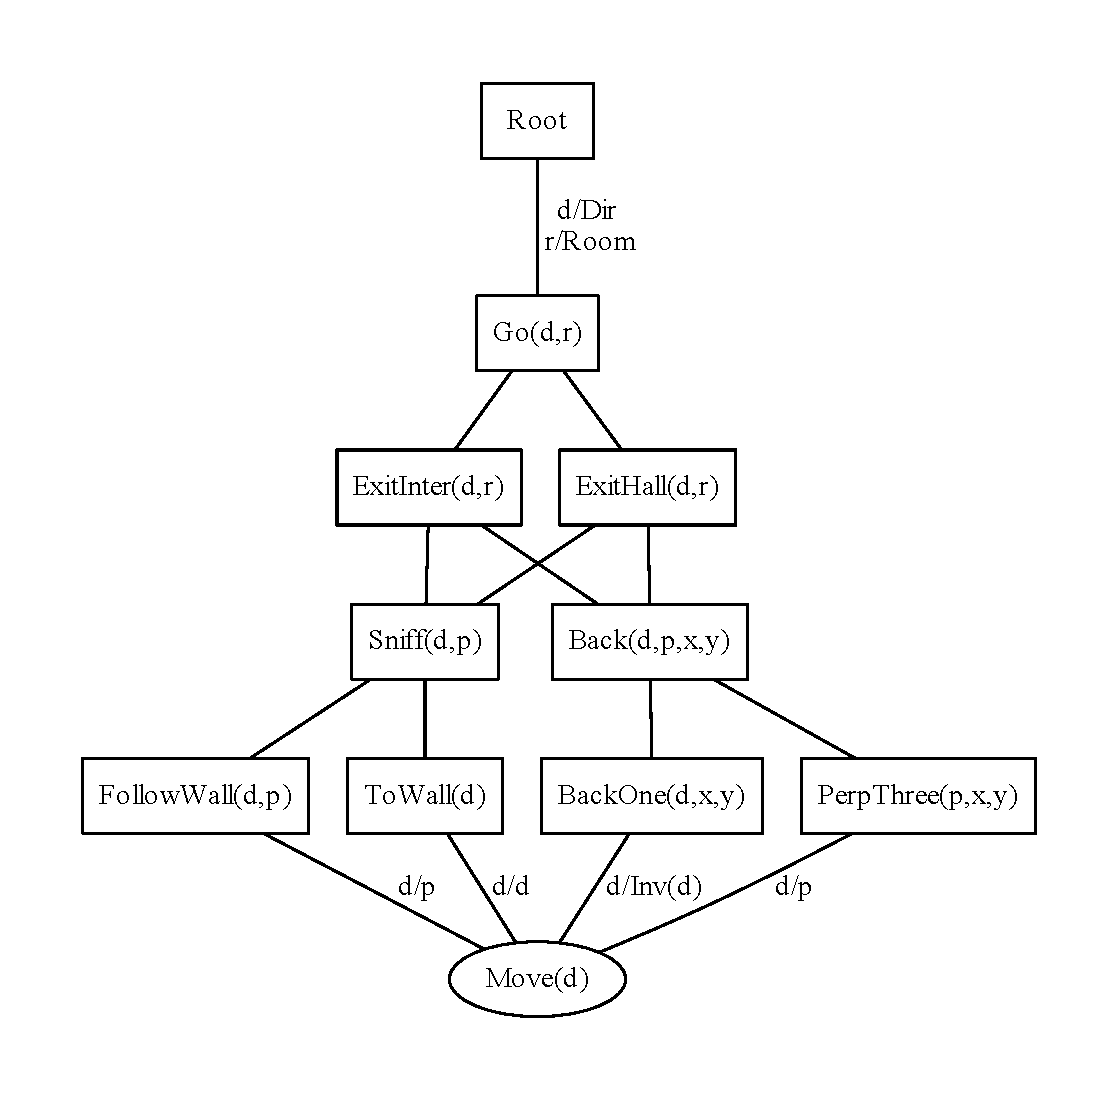
\includegraphics[scale=0.5]{task/Hallway-Hierarchy.pdf}} \\
 \includegraphics[scale=0.27]{task/Taxi-Hierarchy.pdf} & \\
 \includegraphics[scale=0.27]{task/Wargus-Hierarchy.pdf} & \\
 \end{tabular}
 \caption{Task Hierarchies for {\sf Taxi-World} (top-left), {\sf Resource-collection} (bottom-left) and {\sf Hallway} (right). Note that in subtasks Sniff and Back of Hallway, parameter $p$ is perpendicular to $r$, $(x, y)$ is the location of agent when Back is called.}\label{fig:tasks}
 \end{figure*}

%\section{Supplementary experiments}
%We also compare the performance of {\sf B-MaxQ} with pseudo reward learning and {\sf ALispQ} on standard {\sf Taxi-World} domain, where pseudo reward is not needed. Figure~\ref{fig:alisp} shows the results. From the graph, we can see that {\sf B-MaxQ} converges slightly faster than {\sf ALispQ}. In this case, both algorithms try to learn the pseudo reward or external value of subtasks. But {\sf B-MaxQ} learns pseudo rewards only for subtasks with multiple exits (given by prior knowledge), while {\sf ALispQ} has to learn external values for all subtasks. In {\sf Taxi-World}, only subtask ``PUT'' has multiple exits. So less values are required to learn in {\sf B-MaxQ} compared with that in {\sf ALispQ}.
%\begin{figure*}[ht]
%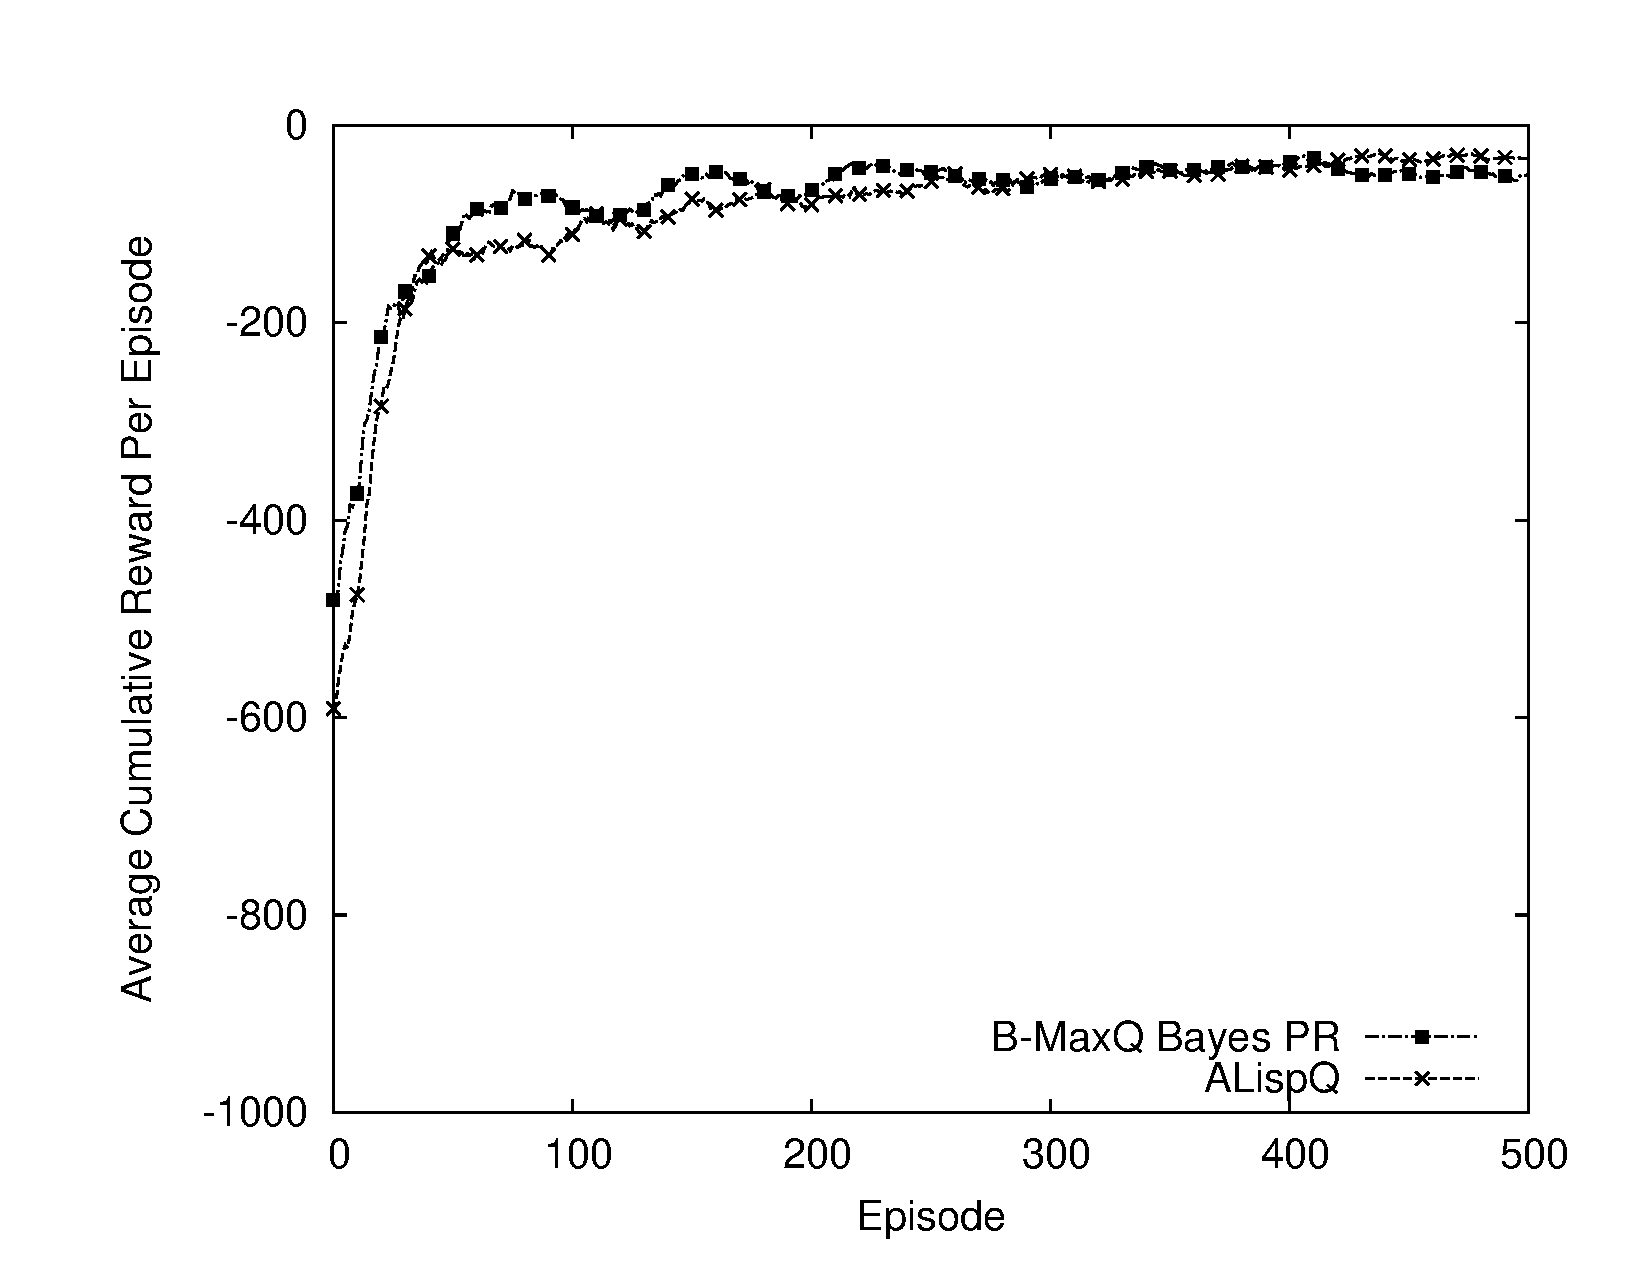
\includegraphics[scale=0.5]{exp/TaxiAlispQ.pdf}
%\caption{Performance of {\sf B-MaxQ} and {\sf ALispQ} on {Taxi-World}.}\label{fig:alisp}
%\end{figure*}


\end{document}



